\section{Обзор и анализ существующих подходов и методов в области обнаружения аномалий}

В данном разделе представлен обзор и сравнительный анализ современных подходов к обнаружению аномалий в контейнерных средах, с акцентом на решения, применяемые в Kubernetes-кластерах. Особое внимание уделяется методам, основанным на использовании нейронных сетей, поскольку именно они в последние годы демонстрируют наибольшую эффективность при обработке сложных, высокоразмерных и временно зависимых данных, характерных для распределённых систем.

В рамках данного раздела рассматриваются три современных решения: GATAKU, KubAnomaly и DeepLog. Выбор этих систем обусловлен тем, что они представляют различные парадигмы применения нейронных сетей для анализа поведения распределённых систем:

\begin{itemize}
    \item использование графовых нейронных сетей (GNN) для моделирования сетевых взаимодействий между компонентами кластера (GATAKU);
    \item применение полносвязных нейронных сетей (MLP) для анализа агрегированных событий мониторинга (KubAnomaly);
    \item использование рекуррентных нейронных сетей (LSTM) для моделирования последовательностей логов и выявления временных аномалий (DeepLog).
\end{itemize}

Для каждого из рассматриваемых решений проводится анализ по следующим критериям:

\begin{itemize}
    \item архитектура модели и используемый тип нейронной сети;
    \item источники входных данных (логи, метрики, сетевые события и др.);
    \item методы предобработки, агрегации и разметки данных;
    \item типы обнаруживаемых аномалий;
    \item применимость в реальных Kubernetes-средах.
\end{itemize}

\subsection{GATAKU}

В работе \cite{Osswald_2025_Anomaly_Detection_Microservices_GNN} рассматривается использование графовых нейронных сетей (GNN) для обнаружения аномалий в кластерах Kubernetes. Авторы предлагают средство обнаружения аномалий на основе GNN в Kubernetes под названием GATAKU (GNN-based Anomaly Detection in Kubernetes). В качестве источников сетевых событий используются CNI-плагин Cilium \cite{cilium} и ingress-контроллер Traefik \cite{Traefik}. Главная цель работы — разработать модель, основанную на графовых нейронных сетях, способную эффективно и точно выявлять потенциальные угрозы и аномалии в кластере Kubernetes на основе сетевых событий.

Тестовая среда представляет собой Kubernetes-кластер, состоящий из 5 узлов: один мастер-узел и четыре рабочих узла. В качестве CNI-плагина использован Cilium совместно с интегрированным сборщиком Hubble, который обеспечивает глубокую наблюдаемость сети и сбор сетевых потоков на уровнях L3–L4 стека TCP/IP.

В кластере развернуто простое многосервисное приложение, включающее:
\begin{enumerate}
    \item \textbf{Frontend}: сервис в двух репликах, доступный из интернета через Traefik Ingress.
    \item \textbf{Backend}: сервис в четырёх репликах, принимающий запросы от Frontend и обращающийся к сервису данных и базе данных.
    \item \textbf{Сервис базы данных} (например, Postgres) в трёх репликах, обрабатывающий запросы от Backend.
    \item \textbf{Сервис Adata}: сервис в двух репликах, принимающий запросы от Backend и отправляющий некоторые запросы во внешние сервисы за пределами кластера.
\end{enumerate}

Поды периодически генерируют трафик с помощью утилиты curl для имитации нормального взаимодействия между сервисами.

Для моделирования аномального трафика авторы рассматривают три сценария атак:

\begin{itemize}
    \item Атаки типа «отказ в обслуживании» (DoS): запускается вредоносный под, который случайным образом выбирает целевой доброкачественный под в том же пространстве имен и начинает отправлять множество HTTP-запросов на него с помощью утилиты hey.
    \item Несанкционированное сканирование портов для атак разведки: сценарий похожий на DoS, только вредоносный порт начинает сканирование портов с помощью утилиты nmap.
    \item Сканирование веб-приложений на веб-уязвимости: запускается инструмент OWASP ZAP, который применяется для сканирования уязвимостей приложения.
\end{itemize}

Разработка GATAKU выполнена в два этапа: сбор данных (запуск сценариев атак в тестовом кластере) и обучение модели с контролируемым обучением для обнаружения аномалий в сетевых данных.

Разработка модели включает три этапа:

\begin{enumerate}
    \item \textbf{Предобработка данных}. Реализован конвейер предобработки, преобразующий каждый признак в числовой или категориальный формат. Использованы различные кодировщики и нормализаторы для IP-адресов, портов, флагов TCP/UDP и других признаков. Помимо исходных характеристик введены дополнительные агрегирующие признаки (по портам, IP-адресам, временным интервалам) для вычисления индексов разнообразия.
    \item \textbf{Построение графа}. Для формирования графовой структуры используется метод $k$-ближайших соседей (kNN): для каждой точки данных находят $k$ наиболее похожих по признакам соседей, после чего каждая точка рассматривается как узел графа с рёбрами к $k$ ближайшим узлам. Такой метод выбран благодаря простоте реализации и пригодности для наборов данных с относительно небольшой размерностью. Авторы подчеркивают, что данный алгоритм хорошо работает на наборах с относительно небольшим числом измерений.
    \item \textbf{Разработка модели НС}. В качестве модели используется графовая сверточная сеть (GCN), представленая на рисунке ~\ref{fig:GATAKU_ML_model}. Архитектура включает три сверточных слоя, слой регуляризации (dropout), функцию активации ReLU в скрытых слоях и Softmax в выходном слое. Модель формирует вероятности принадлежности точки данных к соответствующим классам аномалий.
\end{enumerate}

\begin{figure}
    \centering
    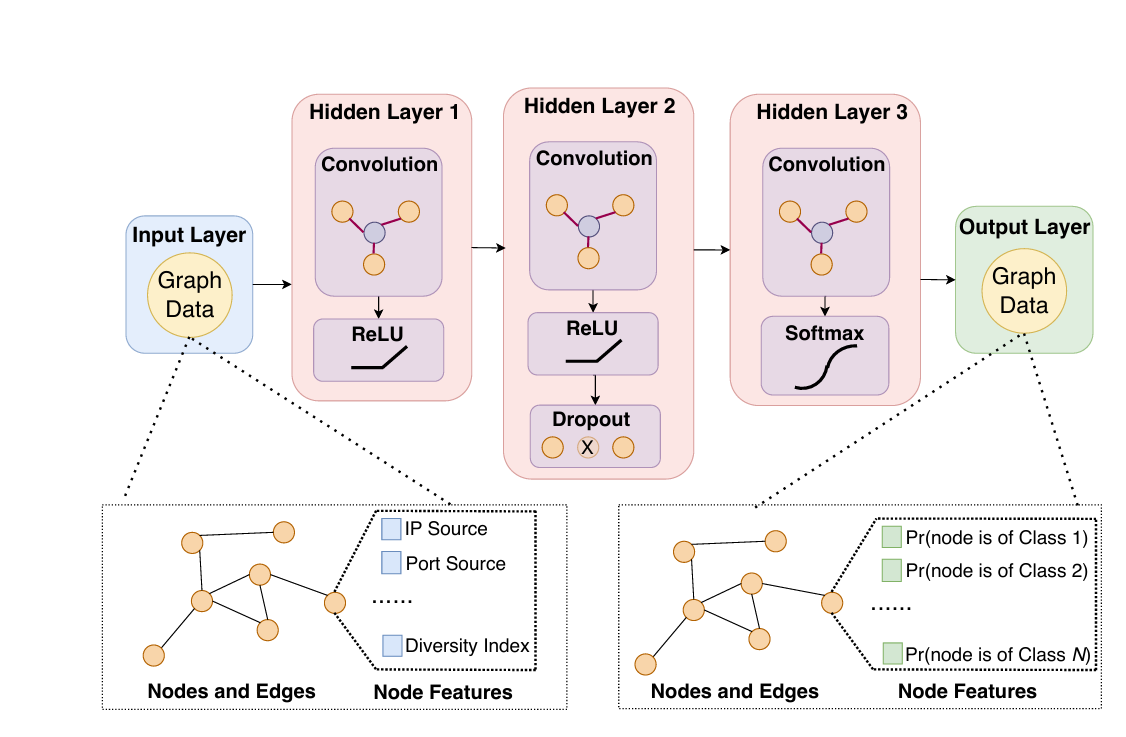
\includegraphics[scale=0.5]{inc/images/GATAKU-ML-model}
    \caption{Обзор модели GCN в GATAKU \cite{Osswald_2025_Anomaly_Detection_Microservices_GNN}.}
    \label{fig:GATAKU_ML_model}
\end{figure}

По результатам экспериментов GATAKU показала небольшое улучшение качества по сравнению с методами RF и SVM. Однако модель подвержена ограничениям по масштабируемости: построение графа (kNN), обучение GCN и обработка графовых структур создают значительную вычислительную нагрузку. Авторы отмечают, что в ресурсно-ограниченных средах применение GNN требует оптимизаций.

\subsection{KubAnomaly}

Авторы исследования \cite{KubAnomaly} предлагают KubAnomaly — систему, обеспечивающую возможности мониторинга безопасности для обнаружения аномалий на платформе оркестрации Kubernetes. Данная система представляет собой модуль мониторинга контейнеров для Kubernetes с использованием НС для создания моделей классификации, которые усиливают способность системы выявлять аномальное поведение, такое как атаки на веб-сервисы, атаки, использующие распространённые и zero-day уязвимости, а также комбинированные атаки на различные компоненты кластера.

KubAnomaly реализует архитектуру с агентами на нодах и централизованным анализатором; основная идея — собирать «сырые» мониторинговые события, агрегировать их в интервалы, строить векторы признаков и классифицировать каждое окно как нормальное или аномальное с помощью обученной модели. Архитектура представлена на рисунке~\ref{fig:KubAnomaly_architecture}.

\begin{figure}
    \centering
    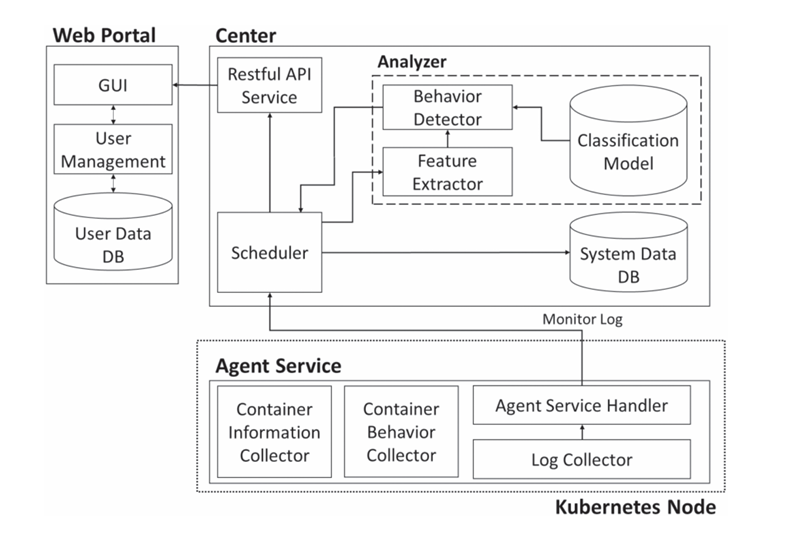
\includegraphics[scale=0.4]{inc/images/KubAnomaly_architecture}
    \caption{Архитектура KubAnomaly \cite{KubAnomaly}.}
    \label{fig:KubAnomaly_architecture}
\end{figure}

Агенты системы KubAnomaly используются для сбора логов мониторинга из контейнеров на основе Docker и также поддерживают Kubernetes. Для сбора событий, описывающих поведение контейнера, используется Falco \cite{falco}. Авторы статьи выделили список событий, которые система отслеживает. Агент отправляет эти данные в центр обработки каждые 10 секунд.

Рабочий процесс KubAnomaly разбит на четыре этапа:

\begin{enumerate}
    \item Сбор логов: агенты отправляют данные в центр обработки каждые 10 секунд.
    \item Извлечение признаков: после получения исходных журналов мониторинга и информации о ПО контейнера журналы преобразуются в нужный формат. Далее исходные журналы мониторинга используются в качестве входных признаков для обучения модели.
    \item Нормализация данных: для увеличения скорости сходимости и точности результата модели МО данные нормализуются.
    \item Построение модели классификации аномалий: модель является полносвязной (fully-connected / MLP) сетью из четырёх слоёв. В качестве функций активации с первого по третий слой используются экспоненциальные линейные единицы (ELU), которые могут ускорять обучение в глубоких нейросетях и обеспечивать более высокую точность классификации. На выходе используется функция Softmax. Исходные данные подаются на первый слой; на выходе возвращается вероятность принадлежности события определённому типу аномалии.
\end{enumerate}

Предложенная модель обнаружения аномалий KubAnomaly может выявлять аномальное поведение контейнеров непосредственно в Kubernetes. Она рассматривается как первая линия защиты для быстрого выявления отклонений. KubAnomaly демонстрирует, что агрегация событий в короткие временные окна и использование нейросетевой классификации дают практичный механизм обнаружения аномалий для контейнерных платформ с высокой точностью на подготовленных наборах данных. Результаты показали, что предложенная модель успешно может выявлять атаки на веб-сервисы с общей точностью до 96\%. При этом решение требует качественно размеченных данных и внимания к производительности агента. Авторы предлагают конфигурации агента и парсинга и показывают, что при аккуратном проектировании накладные расходы остаются приемлемыми.

\subsection{DeepLog}

Авторы работы \cite{DeepLog} предлагают DeepLog — фреймворк для обнаружения аномалий в реальном времени и диагностики на основе системных логов. Идея состоит в том, чтобы рассматривать поток лог-сообщений как последовательность (аналогичную естественному языку), которая следует определенным шаблонам и правилам грамматики, и моделировать её с помощью рекуррентной нейросети LSTM. Данный подход позволяет DeepLog автоматически изучать шаблоны журналов на основе нормального исполнения и обнаруживать аномалии, когда шаблоны журналов отклоняются от модели, обученной на данных журналов при нормальном исполнении. Кроме того авторы предусмотрели постепенное обновление DeepLog в режиме онлайн, чтобы она могла адаптироваться к новым шаблонам журналов со временем.

Для подготовки логов DeepLog сначала парсит неструктурированные текстовые записи и выделяет log key (шаблон сообщения) и параметры (значения), авторы опираются на потоковый парсер Spell для получения структурированного представления логов и идентификации параметров/идентификаторов, позволяющих отделять последовательности, порождённые параллельными задачами.

DeepLog использует не только ключи журналов, но и значения метрик в записи журнала для обнаружения аномалий, благодаря чему способен выявлять разные типы аномалий. В итоге в DeepLog представлено два типа моделей:

\begin{enumerate}
    \item \textbf{Модель аномалий по ключам (Log-Key Anomaly Detection).} Модель на основе LSTM обучается предсказывать следующий лог-ключ по окну предыдущих ключей. В режиме детекции фактический следующий ключ считается аномальным, если он не попадает в множество из top-k наиболее вероятных предсказаний сети (порог k настраиваем). Такой подход эффективно ловит нарушения в порядке и в логике выполнения.
    \item \textbf{Модель аномалий по параметрам (Parameter-Value Anomaly Detection).} Для каждого шаблона логов строится отдельная модель на основе LSTM, моделирующая последовательность векторных параметров/метрик, связанных с этим шаблоном, как мультивариантный временной ряд. Это позволяет выявлять аномалии, связанные с неожиданными значениями параметров или с изменением времени между событиями (performance anomalies).
\end{enumerate}

Общий рабочий цикл DeepLog состоит из двух этапов:

\begin{enumerate}
    \item \textbf{Этап обучения.} Данные для обучения DeepLog представляют собой записи журналов из нормального пути выполнения системы. Каждая запись журнала парсится на ключ журнала и вектор значений параметров. Последовательность ключей журнала, полученная из обучающего файла журнала, используется DeepLog для обучения модели обнаружения аномалий ключей журнала и для построения моделей рабочего процесса выполнения системы в целях диагностики. Для каждого уникального ключа k DeepLog также обучает и поддерживает модель для выявления аномалий, связанных с отклонением от параметров этого ключа.
    \item \textbf{Этап онлайн-детекции.} Новая запись журнала разбивается на ключ журнала и вектор значений параметров. DeepLog сначала использует ключ журнала модель обнаружения аномалий для проверки, является ли входящий ключ лога нормальным. Если да, DeepLog дополнительно проверяет вектор значений параметров с помощью модели обнаружения аномалий значений параметров для этого ключа лога. Новый лог будет помечен как аномалия, если либо его ключ лога, либо предполагается, что его вектор значений параметров является аномальным. Наконец, если Если он помечен как аномальный, модель рабочего процесса DeepLog предоставляет пользователю семантическую информацию для диагностики аномалии. Шаблоны выполнения могут изменяться со временем или не включались в исходные обучающие данные. DeepLog также предоставляет возможность сбора отзывов пользователей. Если пользователь сообщает о обнаруженной аномалии как о ложном срабатывании, DeepLog может использовать это как помеченную запись для поэтапного обновления своих моделей, чтобы учитывать и адаптироваться к новому шаблону.

\end{enumerate}

На рисунке ~\ref{fig:DeepLog_architecture} приведена архитектура DeepLog.

\begin{figure}
    \centering
    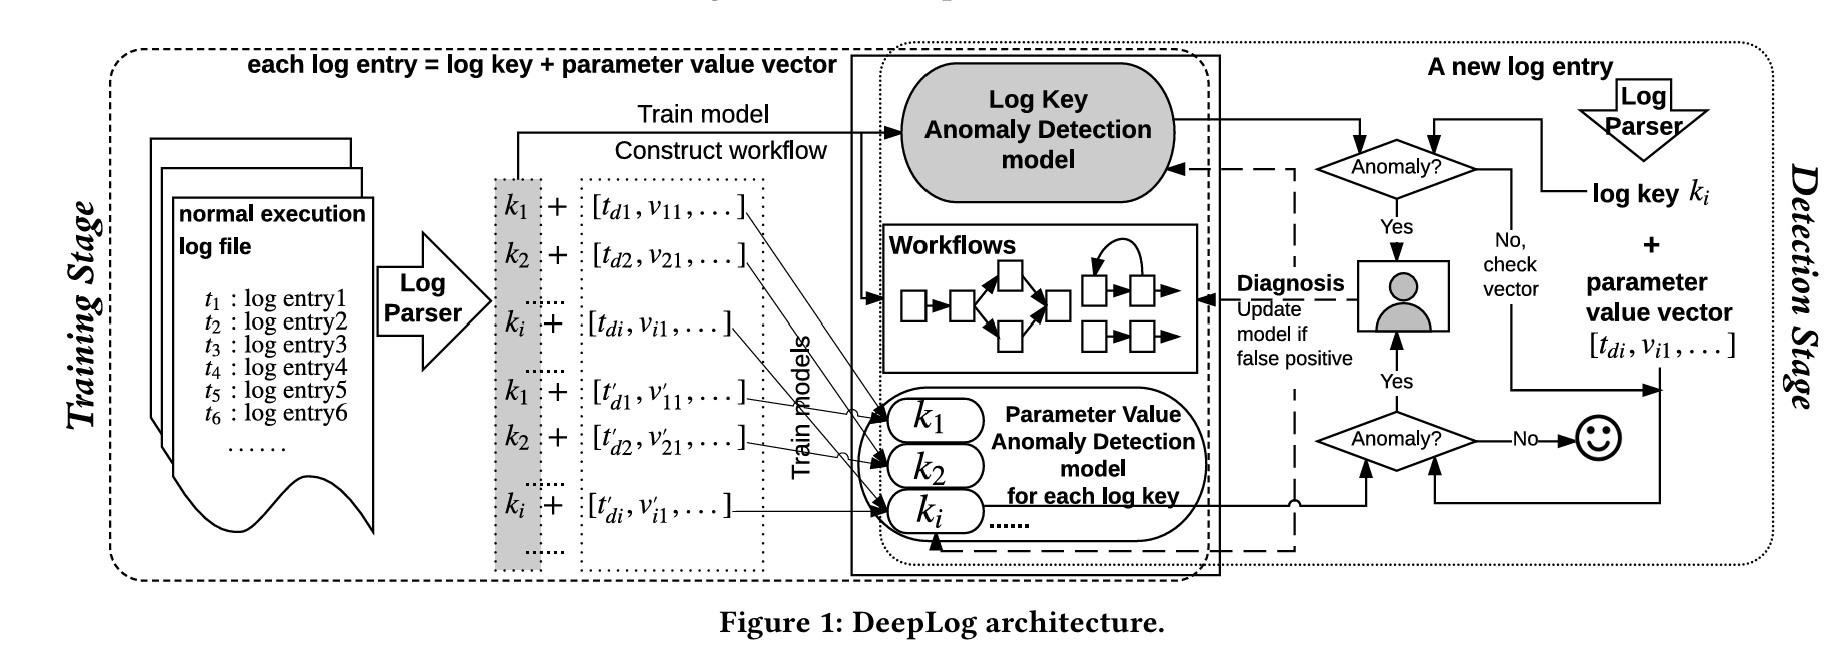
\includegraphics[scale=0.6]{inc/images/DeepLog_architecture}
    \caption{Архитектура DeepLog \cite{DeepLog}.}
    \label{fig:DeepLog_architecture}
\end{figure}

Компоненты DeepLog можно сформулировать схематично следующим образом:

\begin{itemize}
    \item \textbf{Log Parser:} потоковый парсер, преобразующий неструктурированные логи в пары {log key, параметр}, а также выделяющий идентификаторы для группировки записей по «сессиям» или исполнению. Это критический шаг для отделения параллельных потоков исполнения
    \item \textbf{Key Model (LSTM):} многослойная LSTM-сеть, принимающая окно предыдущих ключей и выдающая распределение вероятностей для следующего ключа; используется правило top-k для обнаружения аномалий.
    \item \textbf{Parameter Models (LSTM per key):} для каждого лог-ключа — строится отдельная LSTM-модель, которая анализирует вектор параметров/интервалы между событиями как временной ряд и выявляет аномальные значения или задержки.
    \item \textbf{Workflow Builder / Diagnosis:} модуль, который на этапе обучения конструирует workflow-модели (например, с помощью кластеризации со-встречаемости или на базе предсказаний LSTM) и после детекции использует эти модели для помощи в локализации причины аномалии.
    \item \textbf{Online Updater / Feedback:} механизм инкрементального обновления весов: при ошибочной классификации пользователи могут пометить запись как нормальную, и модель может обновить свои веса онлайн, чтобы адаптироваться к новым шаблонам исполнения.
\end{itemize}

В экспериментальной части авторы показали высокую эффективность DeepLog на нескольких больших наборах логов (включая HDFS и OpenStack): при обучении на очень небольшой доле «чистых» логов (менее 1\%) DeepLog достигает практически 100\% точности обнаружения на оставшейся части HDFS; похожие результаты продемонстрированы и для логов OpenStack. Также проведён анализ влияния параметров (глубины сети, числа юнитов, размера окна h и значения g для top-g), из которого видно, что система относительно устойчива к настройкам и обеспечивает низкую стоимость предсказания (=1 мс на запись на стандартной рабочей станции).

Авторы подчёркивают преимущества DeepLog: способность автоматически изучать сложные порядковые закономерности в логах (благодаря LSTM), интеграция анализа ключей и параметров для более полного покрытия типов аномалий, а также поддержка онлайн-адаптации и инструментов для последующей диагностики. В то же время, как и другие подходы на основе глубокого обучения, DeepLog требует этапа парсинга и достаточного объёма нормальных данных для надёжного обучения, а интерпретируемость отдельных внутренних состояний сети остаётся ограниченной.
